%
% ewsn-full.tex
%

%
% NOTE
%
% ewsn-proc is based on sigplan-proc-varsize 
% The default of sigplan-proc-varsize is 9pt, indented paragraphs (ACM style)
% For EWSN or other 10pt conference, use the 10pt option
\documentclass[10pt,emptycopyrightspace]{ewsn-proc}

% TODO do we really need this?
% % hack to avoid the ugly ACM paragraph definition
% % => can't leave blank line after this
% (remove comment for this hack)
% \renewcommand{\paragraph}[1]{\vskip 6pt\noindent\textbf{#1 }}

\usepackage{graphicx}
\usepackage{graphicx}
\usepackage{balance}
\usepackage{comment}
\usepackage{subcaption}

\newcommand{\fakepar}[1]{\noindent\textbf{#1.}}

\def\sharedaffiliation{%
\end{tabular}\newline
\begin{tabular}{c}}
%
% NOTE
%
% The EWSN reviewing process is double blind: authors must not
% reveal their identities to the reviewers. Names and affiliations
% will only be added for the camera-ready version (see below)
\numberofauthors{1}
\author{
    \alignauthor Saptarshi Hazra,
    Thiemo Voigt,
    Bengt Ahlgren,
    Chenguang Lu,\textsuperscript{*}
    Daniel Cederholm,\textsuperscript{*}
    Gyanesh Patra\textsuperscript{*}\sharedaffiliation
		 \affaddr{RISE SICS, Sweden. \textsuperscript{*}Ericsson Research, Sweden.}\\
		 \affaddr{saptarshi.hazra@ri.se,bengt.ahlgren@ri.se, thiemo.voigt@ri.se,chenguang.lu@ericsson.com}\\
                 \affaddr{daniel.cederholm@ericsson.com,gyanesh.patra@ericsson.com}
}

%\numberofauthors{6}
%\author{
%\alignauthor Double Blind \\
%  \affaddr{do not reveal authors}
%}


%
% NOTE
%
% The command \alignauthor (no curly braces needed) should
% precede each author name, affiliation/snail-mail address and
% e-mail address. Additionally, tag each line of
% affiliation/address with \affaddr, and tag the
%% e-mail address with \email.
%\numberofauthors{2}
%\author{
%\alignauthor Alice User \\
%    \affaddr{University of Southern California}\\
%    \email{alice@example.edu}
%\alignauthor Bob Privacy \\
%    \affaddr{Networked Embedded Systems Group}\\
%    \affaddr{Swedish Institute of Computer Science}\\
%    \email{bob@example.se}
%}


\title{Demo: Multi-Radio Access Technology IoT Gateway}


\begin{document}

\maketitle

%\begin{abstract}
%TV: We may skip the abstract
%This paper provides a sample of a \LaTeX\ document for EWSN. 
%It complements the document \textit{Author's (Alternate) Guide to
%Preparing ACM SIG Proceedings Using \LaTeX$2_\epsilon$\ and Bib\TeX}.
%This source file has been written with the intention of being
%compiled under \LaTeX$2_\epsilon$\ and BibTeX.
%To make best use of this sample document, run it through \texttt{pdflatex}
%and \texttt{bibtex} to directly produce a pdf document.
%\end{abstract}

%
% NOTE
%
% Do not provide category, terms, keywords for the reviewed submission.
% They will only be added for the camera-ready version. Instructions will
% be provided for the camera ready version.

%
% A category with the (minimum) three required fields
% \category{H.4}{Information Systems Applications}{Miscellaneous}
%A category including the fourth, optional field follows...
% \category{D.2.8}{Software Engineering}{Metrics}[complexity measures, performance measures]
% \terms{Delphi theory}
% \keywords{ACM proceedings, \LaTeX, text tagging}

\section{Introduction}
  \label{sec:intro}
Internet of Things (IoT) solutions have been enacted in different application domains independently targeting particular use cases resulting in a plethora of different Radio Access Technologies (RATs) and application architectures. Upcoming challenges particularly in smart cities and industries must provide a combination of these wireless technologies to address different use cases. The lack of integrated infrastructure for convergent access is further exacerbated by the ever increasing number of RATs and the lack of a single solution fitting the requirements of all use cases. 


Traditional approaches have used dedicated radio hardware for different communication technologies. This approach is hard to scale and lacks flexibility. In our previous work, we have introduced VGATE~\cite{hazra2019handling}, a virtual gateway that uses software baseband processing. VGATE uses Software Defined Radios (SDRs) for designing the core baseband functionality as software functions. The functions are implemented as containers on an edge and fog computing infrastructure. This approach makes the baseband functions easy to upgrade to future standard revisions.  It also enables the possibility of deploying the baseband resources based on network load leading to better resource utilization with better energy efficiency.


In this demo, we present a basic implementation of our VGATE architecture incorporating three baseband functions, namely IEEE 802.15.4, LoRa and NB-IoT in a single testbed. We showcase the following:
\begin{itemize}
	\item Simultaneous multi-channel access for IEEE 802.15.4.
	\item Feasibility of our VGATE architecture for providing convergent access.
	\item Feasibility of simultaneously running multiple RATs without loss of performance on the same shared infrastructure.
\end{itemize}

\section{VGATE Design and Implementation}
\label{sec:implementation}
Our VGATE architecture
has two main infrastructure layers: edge and radiohead. The radiohead manages access and transfers radio samples to and from the wireless medium.  The edge hosts the baseband function for each RAT. Both the radiohead and edge functions are virtualized as self-contained containers. In this design, multiple RATs can be simultaneously supported at one shared Edge
infrastructure. %We refer to this design as split setup.


We design the baseband functions to explore necessary methods needed to support the simultaneous operation of multiple RATs on a single shared infrastructure. A cluster of these functions and methods are formed into a container which is deployed on the edge and radiohead. We discuss our software components below. 

\subsection{Radiohead}
The radiohead functions are designed in the GNU Radio framework. The main functionalities are the following:
\begin{itemize}
	\item \textbf{USB-Ethernet conversion}: This performs the interface adaptation from the USB to Ethernet interface. Both TCP and UDP are utilized as transport protocols.
	
	\item \textbf{IQ-sample filtering}: In order to reduce the traffic on the Ethernet, we implement preamble detection on the radiohead. This enables us to suppress unnecessary radio samples and transmit only radio samples that belong to a packet to the edge. 
	
	\item \textbf{ Multi-channel multiplexing/de-multiplexing}: This is implemented for IEEE 802.15.4. It multiplexes multiple channels into a single wideband signal on the downlink. For the uplink, it demultiplexes the wideband signal into radio samples for each individual channel. This is implemented using polyphase filters.
	
\end{itemize}
\subsection{Edge}
The edge hosts the core signal processing functions for each RAT and also the networking stack. The main functionality of the Edge container for each of our RATs are:
\begin{itemize}
	\item \textbf{IEEE 802.15.4}: Contiki-NG provides the network stack for the IEEE 802.15.4 function through a UDP-based radio driver. The CSMA Medium Access Control (MAC) layer is modified to support the increased round trip times introduced by the SDR setup. The physical layer (PHY) is adpated from [] to support our architecture and provides multi channel support. For our demonstration we use a Light Weight Machine to Machine Server (LWM2M) as our application layer. 		
	\item \textbf{LoRa}: We adapt the GNU Radio-based LoRa setup to our architecture and also introduce multi channel support. Our LoRa function supports L1 and simple application layer sending and receiving messages with the Pycom Fife platform.
	

	\item \textbf{NB-IoT}: We implement some key components of the OFDM transmitter for NB-IoT in GNU Radio. A convolutional coding rate of 1/2 is used. We have developed a chat application that supports sending of Telegram messages from a mobile phone to the receiver.
\end{itemize}

% Should there be some description about the demonstration scenario and stuff?
% Not needed

\section{Evaluation}

\begin{figure}[t]
  \vspace{-0.5cm}
  \centering
	\includegraphics[width= 0.42 \textwidth]{setup.png}
	\caption{Evaluation Setup}
	\label{fig:setup}
\end{figure}

\fakepar{Setup} As shown in Figure~\ref{fig:setup}, our evaluation setup includes
three USRPs with the corresponding radioheads that perform the
radiohead functions described above. USRP~1 is configured at 2.4 GHz
band with a sample rate of 15 Msps to cover three 5 MHz channels for
the IEEE 802.15.4 multi-channel implementation. USRP~2 handles NB-IoT;
also at 2.4 GHz but non-overlapped with the IEEE 802.15.4
carriers. The choice of 2.4 GHz is only for test and demonstration
purpose to be able to transmit the RF signal over the air. The sample
rate is set to 1.92 Msps. Finally, USRP~3 is
configured at the EU 863-870 MHz unlicensed band for LoRa. The sample
rate is set to 1Msps to support up to 2 channels.

The radio heads communicate with the edge over Ethernet using UDP. The edge hosts the networking stack including the physical layer. As IoT devices we use a Zolertia Firefly (802.15.4), a LoRa  Pycom FiPy and for NB-IoT, we develop our own NB-IoT receiver emulator using an USRP and a laptop or mini PC, on which implement some key components of NB-IoT receiver functionalities using GNU Radio.

\fakepar{Evaluation}

The goal of this experiments is to show that the
performance of each IoT RAT should not suffer when running with other IoT RATs simultaneously.

Figure~\ref{fig:5-5} shows the ping results in terms of CDF against
the Ping round-trip times (RTT) values and the packet error (PER) in
each RAT combination.  The figure shows increase in PER value when
including additional RATs.  As the execution of IEEE 802.15.4 is
highly computing intensive, the packet error rate (PER) increases
slightly due to the resource contention at the radio head (implemented
in software on a PC) in case of multi-RAT, which is not part of the
Edge. The MAC retransmission timeout for Acknowledgements of
successfully transmitted packets is set to 100ms, which explains the
knee in the curves around that 100ms point in Figure~\ref{fig:5-5}.
In real scenarios, the radio head functions will be implemented in
hardware, e.g. FPGA, DSP etc. which would avoids this
problem. Therefore, the results show that IEEE 802.15.4 can be
realized with same performance in presence of other RATs in our
Multi-RAT IoT scenario.



\begin{figure}[h]
%	\vspace{-0.3cm}
  \centering
	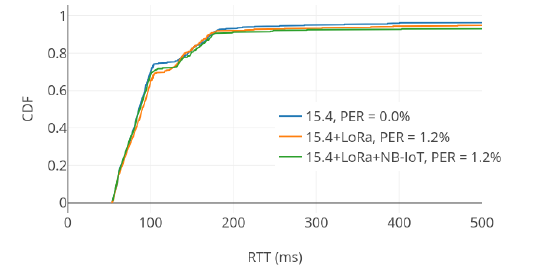
\includegraphics[width= 0.4 \textwidth]{5-5.png}
	\caption{Comparison CDF and RTT of Ping and PER for IEEE
802.15.4 in multi-RAT scenario}
	\label{fig:5-5}
\end{figure}


\begin{figure}[h]
  \vspace{-0.3cm}
	\centering
	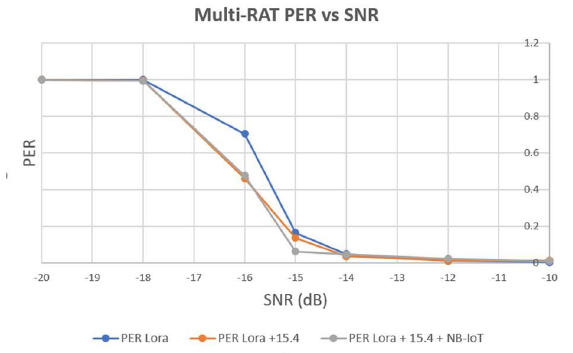
\includegraphics[width= 0.4 \textwidth]{5-6.png}
	\caption{Comparison PER vs SNR for LoRa in multi-rat scenario, SF = 7
}
	\label{fig:5-6}
\end{figure}


Figure~\ref{fig:5-6} shows the PER vs SNR results for LoRa in a
multi-RAT scenario. In this experiment, the LoRa received signal power
is kept constant at -28dBm and noise is added in the radio head
software to for SNR configuration to obtain a specific value of
SNR. The Pycom FiPy continuously transmits 500 data packets with SF =
7 and at the edge we count the number of received packets for
different SNRs. Figure 5-6 shows that the results are very similar
among three scenarios for single, two and three RATs running
simultaneously, respectively. The results indicate that the performance of our
LoRa receiver is not affected by the presence of other RATs with all
the combinations showing close to 0\% PER when SNR is set greater than
-10dB.

\fakepar{Summary} We have presented VGATE, a multi-RAT IoT gateway.
Our results indicate that with VGATE, multiple RATs can be
simultaneously supported at one shared edge infrastructure
with little impact on protocol performance.


%TV: did not get this to work...always went on 3rd page
%\begin{figure*}[th]
%	\centering
%	\begin{subfigure}[t]{.3\textwidth}
%	    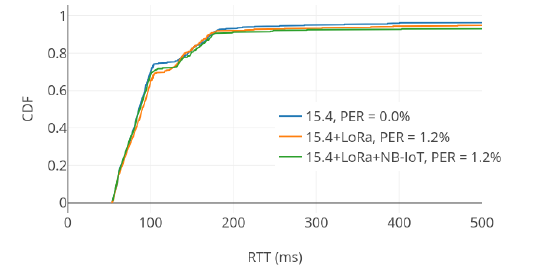
\includegraphics[width=\columnwidth]{5-5.png}
%	  	\caption{Original example of a two tap}
%	  	\label{fig:5-5}
%	\end{subfigure}
%	~
%	\begin{subfigure}[t]{.3\textwidth}
%		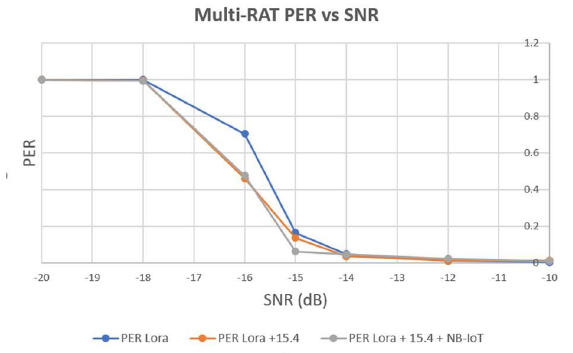
\includegraphics[width=\columnwidth]{5-6.png}
%		\caption{A two tap keeping only every 20th sample with interpolation}
%		\label{fig:5-5}
%	\end{subfigure}
%\end{figure*}



%
% NOTE
%
% The following commands are all you need in the
% initial runs of your .tex file to
% produce the bibliography for the citations in your paper.
\balance
\bibliographystyle{abbrv}
\bibliography{sigproc}  % sigproc.bib is the name of the Bibliography in this case
\end{document}
